\documentclass{standalone}
\usepackage{tikz}
\usetikzlibrary{shapes.geometric}

\begin{document}

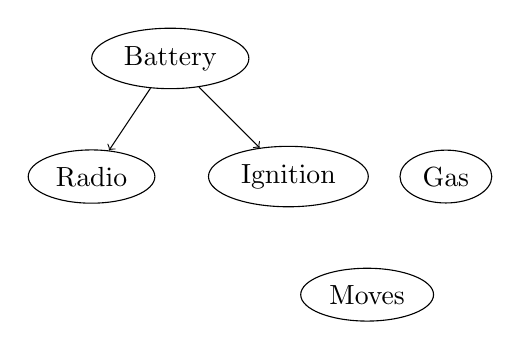
\begin{tikzpicture}
    \node[shape=ellipse,draw=black] (Battery) at (-2,5) {Battery};
    \node[shape=ellipse,draw=black] (Radio) at (-3,3.5) {Radio};
    \node[shape=ellipse,draw=black] (Ignition) at (-0.5,3.5) {Ignition};
    \node[shape=ellipse,draw=black] (Gas) at (1.5,3.5) {Gas};
    \node[shape=ellipse,draw=black] (Moves) at (0.5,2) {Moves};

    \path [->] (Battery)  edge node[below] {}  (Radio);
    \path [->] (Battery)  edge node[below] {}  (Ignition);
%    \path [->] (Ignition) edge node[below] {}  (Moves);
%    \path [->] (Gas)      edge node[below] {}  (Moves);
\end{tikzpicture}

\end{document}